\section{Agreement}\label{sec:agreement}
%% FUNCTION: Shows that round robin achieves EFX less often in a world where agents agree more on
%% what is valuable, first in the reference cell, then as a count over all cells. The only proven
%% case, full agreement without divisibility, is deferred to Section 4.4. Survival curves show
%% that failures also become more severe. Because the size of the effect depends on how far
%% values are spread, the next section turns to dispersion.

\subsection{EFX Rate}\label{sec:agreement-rate}

\begin{figure}[H]
  \centering
  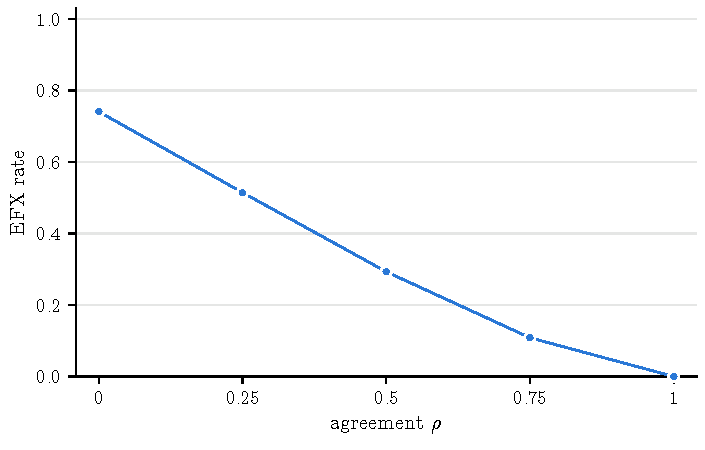
\includegraphics{fig41_agreement_rate.pdf}
  \caption{EFX rate of Round Robin against agreement $\rho$, for $n=4$ agents, $m=12$ goods and dispersion
  $\theta=1$. Each point rests on $R=20{,}000$ instances. The line between the points is for
  illustration only.}
  \label{fig:agreement}
\end{figure}

\subsection{Severity of Failures}\label{sec:agreement-severity}

\begin{figure}[H]
  \centering
  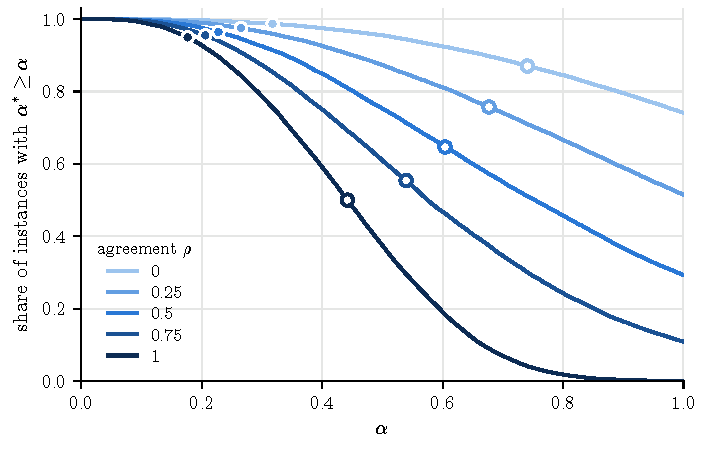
\includegraphics{fig41_agreement_survival.pdf}
  \caption{Share of instances with $\astar\geq\alpha$ under Round Robin, one curve per level of agreement
  $\rho$, for $n=4$ agents, $m=12$ goods and dispersion $\theta=1$. Each curve rests on
  $R=20{,}000$ instances and ends at $\alpha=1$ in the EFX rate. The filled point on each curve
  marks the $5\%$ quantile and the open point the median of $\astar$ among the instances that
  are not EFX.}
  \label{fig:agreement-survival}
\end{figure}

